


\subsection{Evaluation}
We picked two representative bug kernels \texttt{etcd7443} and \texttt{kubernetes11298} to evaluate the coverage idea on them as they
%
They both have extensive use of channels, mutexes, conditional variables, nested selects within nested for loops and the buggy interleaving is proved to be rare to happen.
%
figures \ref{etcd_coverage} and \ref{fig:kubernetes_coverage} show the gradual increase in coverage percentage during execution runs for different values of D.
%
Recall that D is the bound on the number of yields that we inject to the native execution of a given program to perturb the scheduler around concurrency usages.
%
These figures show that
%

\begin{figure}
\centering
  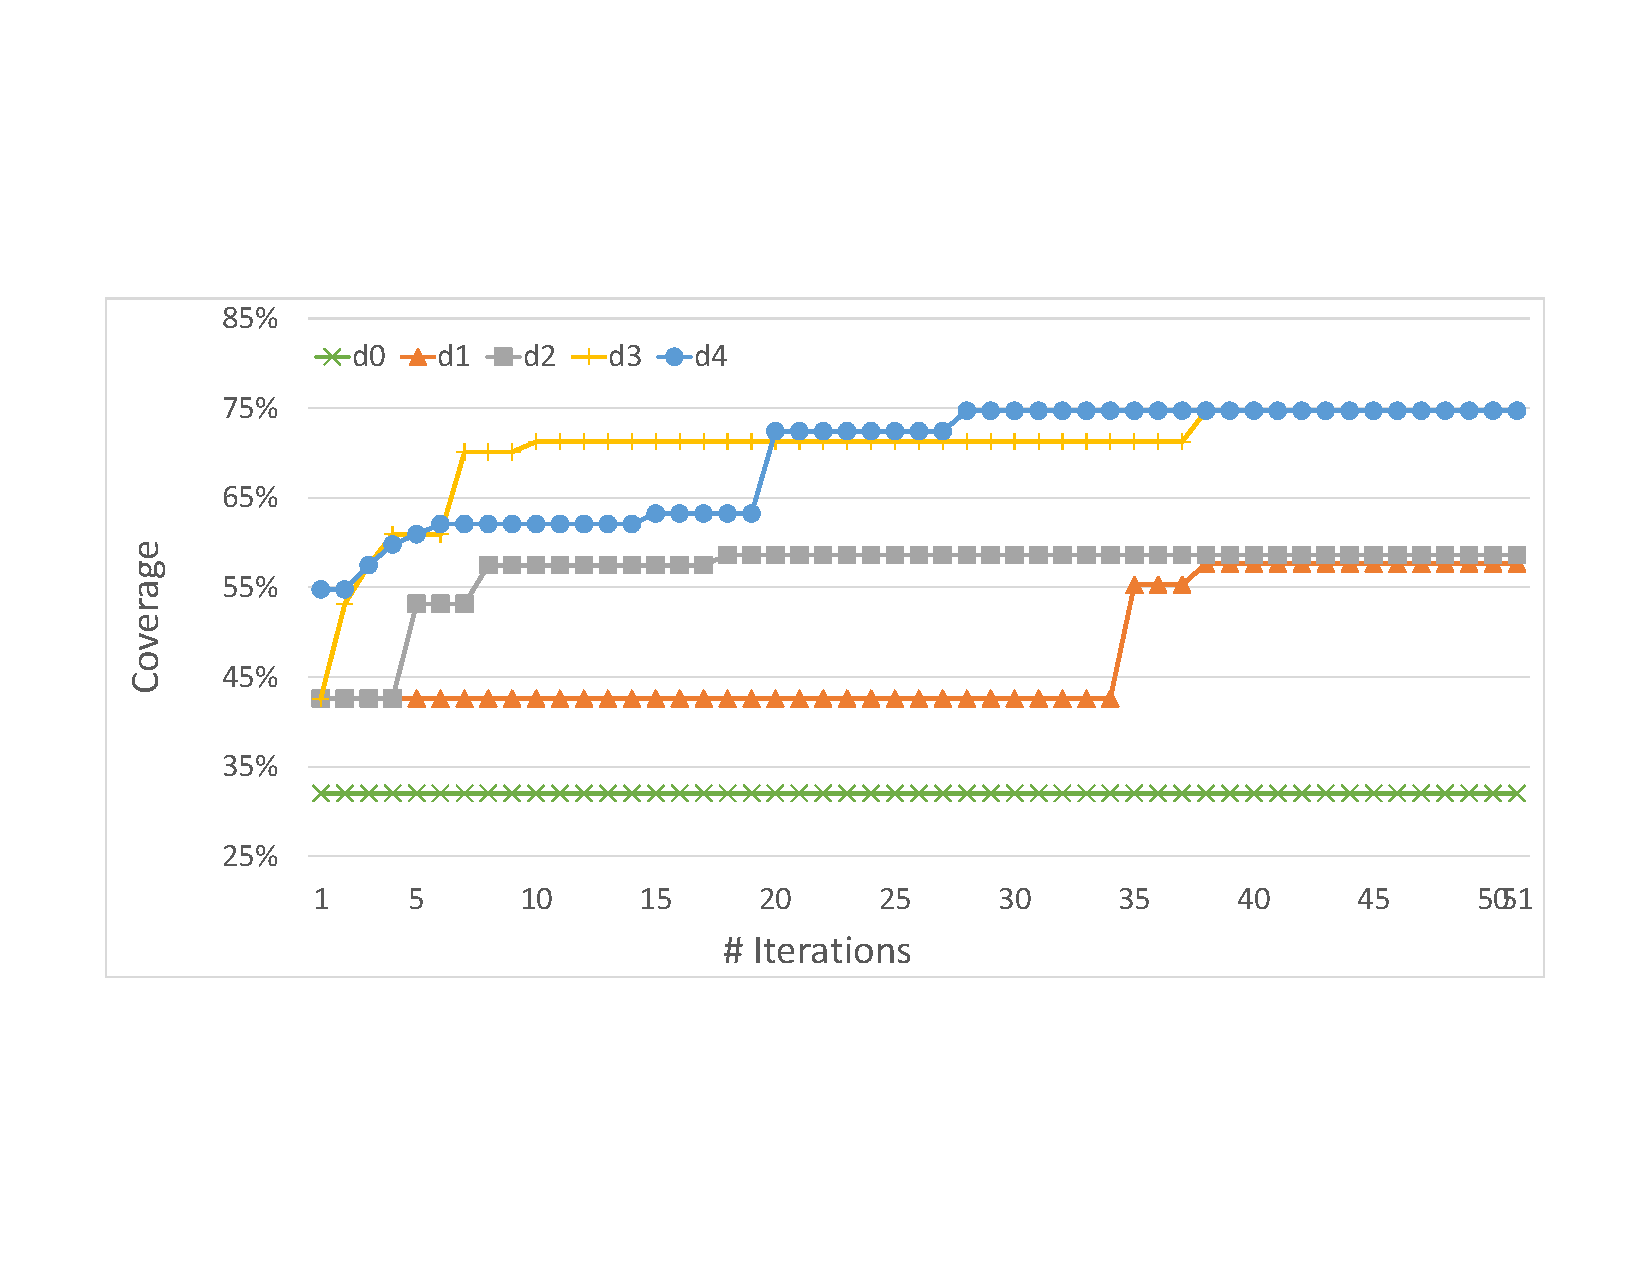
\includegraphics[width=.95\linewidth]{figs/coverage_etcd7443.pdf}
  \caption{etcd7442 coverage}
  \label{fig:etcd_coverage}
\end{figure}


\begin{figure}
\centering
  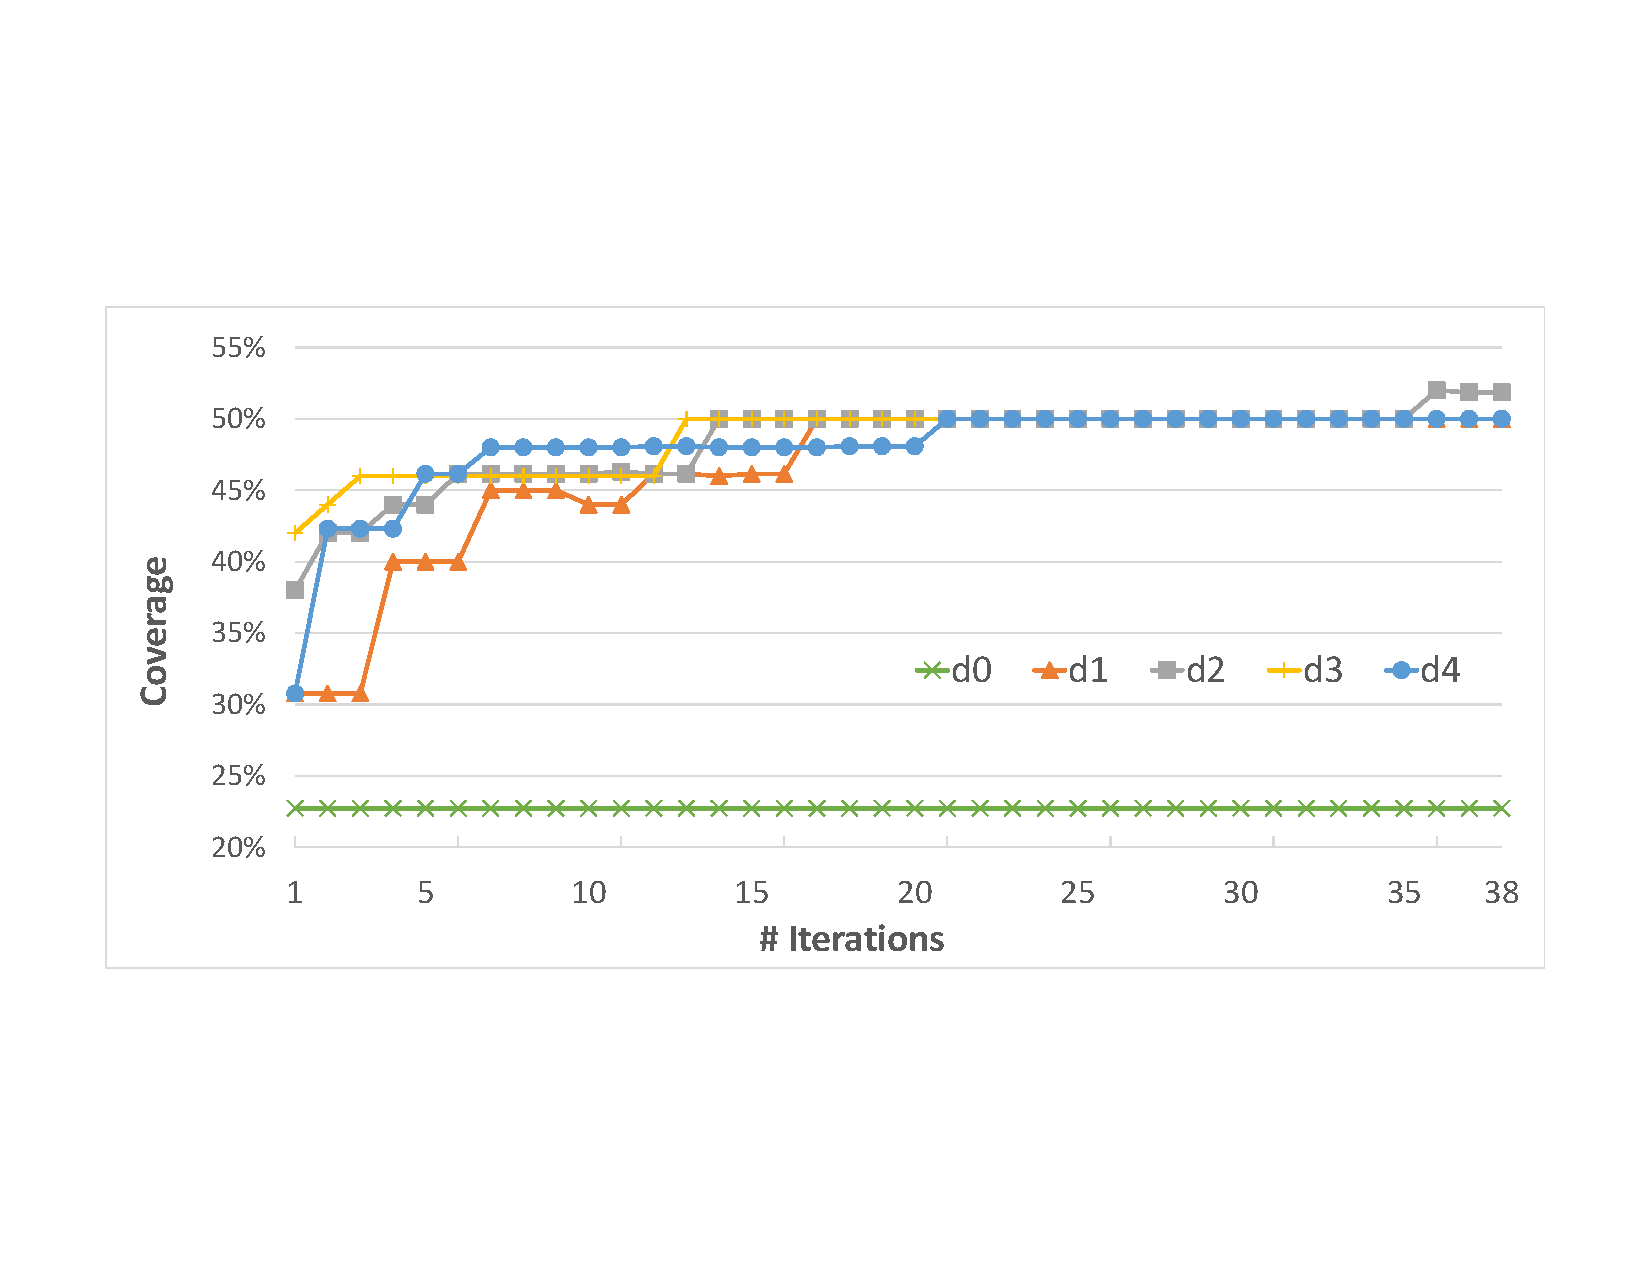
\includegraphics[width=.95\linewidth]{figs/coverage_kubernetes11298.pdf}
  \caption{kuberenetes11298 coverage}
  \label{fig:kubernetes_coverage}
\end{figure}
